\documentclass[border=10pt]{standalone}
\usepackage{tikz}

\begin{document}

\tikzset{every picture/.style={line width=0.75pt}} %set default line width to 0.75pt        

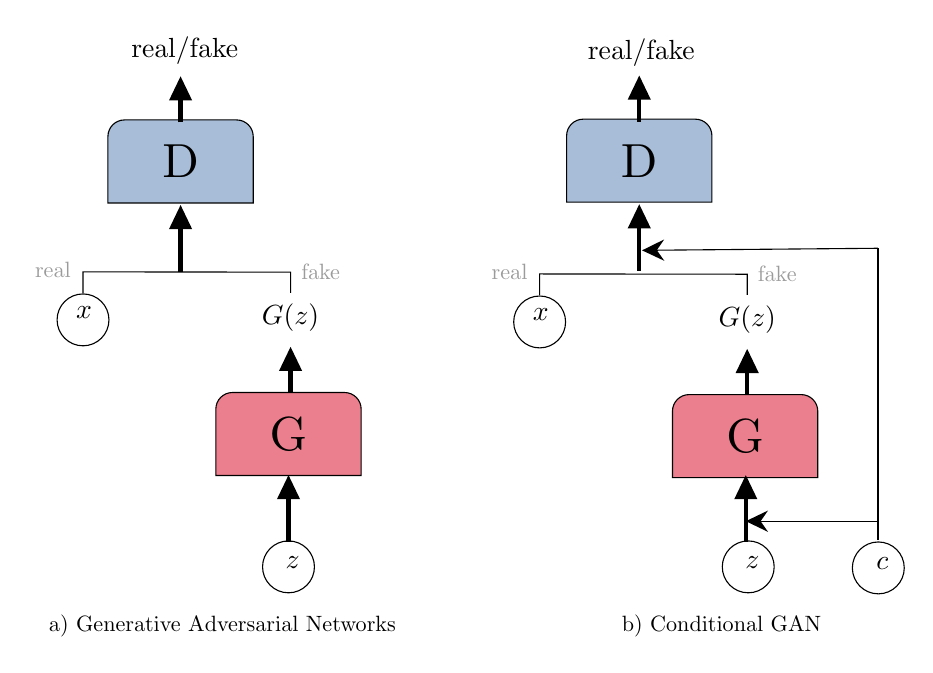
\begin{tikzpicture}[x=0.75pt,y=0.75pt,yscale=-1,xscale=1]
    %uncomment if require: \path (0,300); %set diagram left start at 0, and has height of 300

    %Rounded Same Side Corner Rect [id:dp09824487187603104] 
    \draw  [fill={rgb, 255:red, 167; green, 189; blue, 216 }  ,fill opacity=1 ] (59,53.17) .. controls (59,48.75) and (62.58,45.17) .. (67,45.17) -- (121,45.17) .. controls (125.42,45.17) and (129,48.75) .. (129,53.17) -- (129,85.17) .. controls (129,85.17) and (129,85.17) .. (129,85.17) -- (59,85.17) .. controls (59,85.17) and (59,85.17) .. (59,85.17) -- cycle ;

    %Straight Lines [id:da3936283121049964] 
    \draw [line width=1.5]    (94,46.37) -- (94,27.17) ;
    \draw [shift={(94,24.17)}, rotate = 450] [fill={rgb, 255:red, 0; green, 0; blue, 0 }  ][line width=1.5]  [draw opacity=0] (11.61,-5.58) -- (0,0) -- (11.61,5.58) -- cycle    ;

    %Straight Lines [id:da20962861468486604] 
    \draw [line width=1.5]    (94,108.37) -- (94,89.17) ;
    \draw [shift={(94,86.17)}, rotate = 450] [fill={rgb, 255:red, 0; green, 0; blue, 0 }  ][line width=1.5]  [draw opacity=0] (11.61,-5.58) -- (0,0) -- (11.61,5.58) -- cycle    ;


    %Rounded Same Side Corner Rect [id:dp23742764202945832] 
    \draw  [fill={rgb, 255:red, 236; green, 127; blue, 141 }  ,fill opacity=1 ] (111,184.5) .. controls (111,180.08) and (114.58,176.5) .. (119,176.5) -- (173,176.5) .. controls (177.42,176.5) and (181,180.08) .. (181,184.5) -- (181,216.5) .. controls (181,216.5) and (181,216.5) .. (181,216.5) -- (111,216.5) .. controls (111,216.5) and (111,216.5) .. (111,216.5) -- cycle ;

    %Shape: Circle [id:dp9124405398322727] 
    \draw   (133.5,260.5) .. controls (133.5,253.6) and (139.1,248) .. (146,248) .. controls (152.9,248) and (158.5,253.6) .. (158.5,260.5) .. controls (158.5,267.4) and (152.9,273) .. (146,273) .. controls (139.1,273) and (133.5,267.4) .. (133.5,260.5) -- cycle ;

    %Straight Lines [id:da13727591026438046] 
    \draw    (47,128.5) -- (47,118.37) -- (147,118.5) -- (147,128.5) ;


    %Shape: Circle [id:dp18766521903761446] 
    \draw   (34.5,141.5) .. controls (34.5,134.6) and (40.1,129) .. (47,129) .. controls (53.9,129) and (59.5,134.6) .. (59.5,141.5) .. controls (59.5,148.4) and (53.9,154) .. (47,154) .. controls (40.1,154) and (34.5,148.4) .. (34.5,141.5) -- cycle ;

    %Straight Lines [id:da802599291550045] 
    \draw [line width=1.5]    (147,176.7) -- (147,157.5) ;
    \draw [shift={(147,154.5)}, rotate = 450] [fill={rgb, 255:red, 0; green, 0; blue, 0 }  ][line width=1.5]  [draw opacity=0] (11.61,-5.58) -- (0,0) -- (11.61,5.58) -- cycle    ;

    %Straight Lines [id:da6629044704219691] 
    \draw [line width=1.5]    (94,108.37) -- (94,118.37) ;


    %Rounded Same Side Corner Rect [id:dp8414166975508496] 
    \draw  [fill={rgb, 255:red, 167; green, 189; blue, 216 }  ,fill opacity=1 ] (280,52.8) .. controls (280,48.38) and (283.58,44.8) .. (288,44.8) -- (342,44.8) .. controls (346.42,44.8) and (350,48.38) .. (350,52.8) -- (350,84.8) .. controls (350,84.8) and (350,84.8) .. (350,84.8) -- (280,84.8) .. controls (280,84.8) and (280,84.8) .. (280,84.8) -- cycle ;

    %Straight Lines [id:da2585894594076309] 
    \draw [line width=1.5]    (315,46) -- (315,26.8) ;
    \draw [shift={(315,23.8)}, rotate = 450] [fill={rgb, 255:red, 0; green, 0; blue, 0 }  ][line width=1.5]  [draw opacity=0] (11.61,-5.58) -- (0,0) -- (11.61,5.58) -- cycle    ;

    %Straight Lines [id:da46888126052976953] 
    \draw [line width=1.5]    (315,108) -- (315,88.8) ;
    \draw [shift={(315,85.8)}, rotate = 450] [fill={rgb, 255:red, 0; green, 0; blue, 0 }  ][line width=1.5]  [draw opacity=0] (11.61,-5.58) -- (0,0) -- (11.61,5.58) -- cycle    ;

    %Straight Lines [id:da8917552789067931] 
    \draw [line width=1.5]    (315,108) -- (315,118) ;



    %Rounded Same Side Corner Rect [id:dp5374022902949864] 
    \draw  [fill={rgb, 255:red, 236; green, 127; blue, 141 }  ,fill opacity=1 ] (331,185.5) .. controls (331,181.08) and (334.58,177.5) .. (339,177.5) -- (393,177.5) .. controls (397.42,177.5) and (401,181.08) .. (401,185.5) -- (401,217.5) .. controls (401,217.5) and (401,217.5) .. (401,217.5) -- (331,217.5) .. controls (331,217.5) and (331,217.5) .. (331,217.5) -- cycle ;

    %Shape: Circle [id:dp15401041449631925] 
    \draw   (355,260.5) .. controls (355,253.6) and (360.6,248) .. (367.5,248) .. controls (374.4,248) and (380,253.6) .. (380,260.5) .. controls (380,267.4) and (374.4,273) .. (367.5,273) .. controls (360.6,273) and (355,267.4) .. (355,260.5) -- cycle ;

    %Straight Lines [id:da7442630597870975] 
    \draw    (267,129.5) -- (267,119.37) -- (367,119.5) -- (367,129.5) ;


    %Shape: Circle [id:dp5737171836404196] 
    \draw   (254.5,142.5) .. controls (254.5,135.6) and (260.1,130) .. (267,130) .. controls (273.9,130) and (279.5,135.6) .. (279.5,142.5) .. controls (279.5,149.4) and (273.9,155) .. (267,155) .. controls (260.1,155) and (254.5,149.4) .. (254.5,142.5) -- cycle ;

    %Straight Lines [id:da4180267705785833] 
    \draw [line width=1.5]    (367,177.7) -- (367,158.5) ;
    \draw [shift={(367,155.5)}, rotate = 450] [fill={rgb, 255:red, 0; green, 0; blue, 0 }  ][line width=1.5]  [draw opacity=0] (11.61,-5.58) -- (0,0) -- (11.61,5.58) -- cycle    ;

    %Shape: Circle [id:dp1910511651314143] 
    \draw   (417.67,261) .. controls (417.67,254.1) and (423.26,248.5) .. (430.17,248.5) .. controls (437.07,248.5) and (442.67,254.1) .. (442.67,261) .. controls (442.67,267.9) and (437.07,273.5) .. (430.17,273.5) .. controls (423.26,273.5) and (417.67,267.9) .. (417.67,261) -- cycle ;
    %Straight Lines [id:da4651457466304051] 
    \draw    (430,107) -- (430,247.5) ;


    %Straight Lines [id:da5203121766050092] 
    \draw [line width=1.5]    (366.33,238.5) -- (366.33,219.3) ;
    \draw [shift={(366.33,216.3)}, rotate = 450] [fill={rgb, 255:red, 0; green, 0; blue, 0 }  ][line width=1.5]  [draw opacity=0] (11.61,-5.58) -- (0,0) -- (11.61,5.58) -- cycle    ;

    %Straight Lines [id:da937462245399049] 
    \draw [line width=1.5]    (366.33,238.5) -- (366.33,248.5) ;



    %Straight Lines [id:da9479077607901114] 
    \draw    (368.33,238.5) -- (430,238.5) ;

    \draw [shift={(366.33,238.5)}, rotate = 0] [fill={rgb, 255:red, 0; green, 0; blue, 0 }  ][line width=0.75]  [draw opacity=0] (10.72,-5.15) -- (0,0) -- (10.72,5.15) -- (7.12,0) -- cycle    ;
    %Straight Lines [id:da5439740708699127] 
    \draw    (318.33,107.98) -- (430,107) ;

    \draw [shift={(316.33,108)}, rotate = 359.5] [fill={rgb, 255:red, 0; green, 0; blue, 0 }  ][line width=0.75]  [draw opacity=0] (10.72,-5.15) -- (0,0) -- (10.72,5.15) -- (7.12,0) -- cycle    ;
    %Straight Lines [id:da9106477946558591] 
    \draw [line width=1.5]    (146,238.5) -- (146,219.3) ;
    \draw [shift={(146,216.3)}, rotate = 450] [fill={rgb, 255:red, 0; green, 0; blue, 0 }  ][line width=1.5]  [draw opacity=0] (11.61,-5.58) -- (0,0) -- (11.61,5.58) -- cycle    ;

    %Straight Lines [id:da3221761369788204] 
    \draw [line width=1.5]    (146,238.5) -- (146,248.5) ;




    % Text Node
    \draw (146,196.5) node [scale=1.7280000000000002] [align=left] {G};
    % Text Node
    \draw (147,140.5) node   {$G( z)$};
    % Text Node
    \draw (148,258.5) node   {$z$};
    % Text Node
    \draw (94,65.17) node [scale=1.7280000000000002] [align=left] {D};
    % Text Node
    \draw (161.5,118.5) node [scale=0.8,color={rgb, 255:red, 155; green, 155; blue, 155 }  ,opacity=1 ] [align=left] {fake};
    % Text Node
    \draw (32.5,117.5) node [scale=0.8,color={rgb, 255:red, 155; green, 155; blue, 155 }  ,opacity=1 ] [align=left] {real};
    % Text Node
    \draw (47.5,138) node   {$x$};
    % Text Node
    \draw (96,11.83) node  [align=left] {real/fake};
    % Text Node
    \draw (114.17,289) node [scale=0.8] [align=left] {a) Generative Adversarial Networks};
    % Text Node
    \draw (367,141.5) node   {$G( z)$};
    % Text Node
    \draw (381.5,119.5) node [scale=0.8,color={rgb, 255:red, 155; green, 155; blue, 155 }  ,opacity=1 ] [align=left] {fake};
    % Text Node
    \draw (252.5,118.5) node [scale=0.8,color={rgb, 255:red, 155; green, 155; blue, 155 }  ,opacity=1 ] [align=left] {real};
    % Text Node
    \draw (316,12.83) node  [align=left] {real/fake};
    % Text Node
    \draw (354.67,289) node [scale=0.8] [align=left] {b) Conditional GAN};
    % Text Node
    \draw (267.5,139) node   {$x$};
    % Text Node
    \draw (369.5,258.5) node   {$z$};
    % Text Node
    \draw (366,197.5) node [scale=1.7280000000000002] [align=left] {G};
    % Text Node
    \draw (315,64.8) node [scale=1.7280000000000002] [align=left] {D};
    % Text Node
    \draw (432.17,259) node   {$c$};

\end{tikzpicture}



\end{document}
